% Generalization H : forecasting a slice of the trajectory
\begin{comment}
\subsection{Trajectory Forecasting (NO + FMM)}
\noindent We propose further generalization of our operator so that it maps any point of the trajectory $\mathbf{x}_{t_{n1}}$ to the trajectory between $[\mathbf{x}_{t_{n1}}, \mathbf{x}_{t_{n2}}]$, provided that $t_{n1} > t_{n2}$:
\begin{align}
\mathcal{H}_{\theta} : (\mathbb{R}^d, \mathcal{T}, \mathcal{T}) & \mapsto \mathbb{R}^{N \times d}\\
   \mathcal{H}_{\theta}(\mathbf{x}_{t_{n1}}, t_{n1}, t_{n2}) &= Z_{N - {n_1}} \cup \left\{\widehat{\mathbf{x}}_{t_k}\right\}_{k \in [n_2, n_1 ]} \cup Z_{{n_2} - 1} \\
   & \forall \; (t_{n1}, t_{n2}) \in (\mathcal{T} \setminus \epsilon)^2 \: \: \text{and} \: \: n1 > n2 \label{Hstar:def}\\
   \mathcal{H}_{\theta}(\mathbf{x}_{\epsilon}, \epsilon, \epsilon) &= Z_{N - 1} \cup \mathbf{x}_{\epsilon}  \label{H:bound} \: \: \text{(Boundary Condition)} \\
    \mathcal{H}_{\theta}(\mathbf{x}_{t_n}, t_n, t_n) &= Z_{N - n} \cup \mathbf{x}_{t_n} \cup Z_{n - 1}  \: \: \text{(Identity Mapping)} \\
\end{align}

\noindent The remaining trajectory (between $]\mathbf{x}_{t_{n_2}}, \mathbf{x}_{\epsilon}]$) is set to 0 using $Z_{{n_2} - 1}$. A visual summary of our operator is shown on Figure~\ref{fig:fmmno}\\

\begin{figure}[htbp]
  \centering
  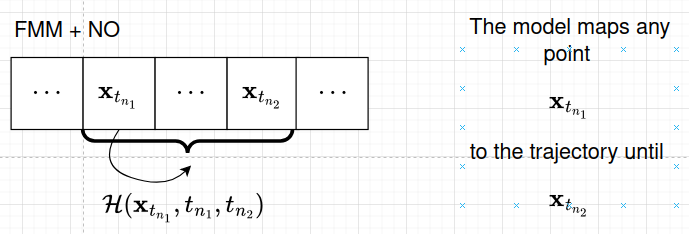
\includegraphics[width=0.5\textwidth]{figures/fmmno.png}
  \caption{A visual summary of our proposal approach.}
  \label{fig:fmmno}
\end{figure}
\end{comment}


% Consistency for operator G
\section{Consistency}
\subsection{Operator $\mathcal{G}$}
\noindent We propose to enforce consistency for all points of the foretasted trajectory:
\begin{align}
    \mathcal{G}\left(\mathbf{x}_{t_{n_1}}, t_{n_1} \right)[\epsilon:n_2] & = \mathcal{G}\left(\mathbf{x}_{t_{n_2}}, t_{n_2} \right),\:\:\:\: (t_{n_1}, t_{n_2}) \in \mathcal{T}^2 \: \text{s.t.} \: t_{n_1} \geq t_{n_2} \\
    \Leftrightarrow \mathcal{G}\left(\mathbf{x}_{t_{n_1}}, t_{n_1} \right) &= \mathcal{G}\left(\mathbf{x}_{t_{n_2}}, t_{n_2} \right) \cup \{\widehat{\mathbf{x}}_{k}^{\phi}\}_{k \in ]t_{n_2}:t_{n_1}]} \label{G:consistency}
\end{align}

% Consistency for operator H
\subsection{Operator $\mathcal{H}$}
\noindent We propose to enforce consistency for all points of the foretasted trajectory that intersect:
\begin{align}
    \mathcal{G}\left(\mathbf{x}_{t_{n_1}}, t_{n_1}, t_{n_2} \right)[\tau] & = \mathcal{G}\left(\mathbf{x}_{t_{n_1}^{'}}, t_{n_1}^{'}, t_{n_2}^{'} \right)[\tau] \\
    \text{with} \: \: \tau & = [t_{n_1}, t_{n_2}] \cap [t_{n_1}^{'}, t_{n_2}^{'}] \label{G:consistency}
\end{align}


\begin{comment}
\noindent The original consistency loss is:
\begin{align}
\mathcal{L}_{\text{CD}}(\theta,\theta^{-}; \phi)
=\frac{1}{n_s}\sum_{k=1}^{n_s}\frac{1}{N}\sum_{i=1}^{N}
\left\lVert f_\theta \left(\mathbf{x}_i^{k} \right)-\operatorname{sg}\!\left(f_{\theta^{-}}\left(\mathbf{x}_i^{\dagger,k}\right)\right)\right\rVert .
\end{align}

\begin{align}
\mathcal{L}_{\text{CD}}(\theta,\theta^{-}; \phi) &= \mathbb{E}\left[\lambda(t_n)d\left(f_{\theta}(\mathbf{x}_{t_{n+1}}), f_{\theta^{-}}(\widehat{\mathbf{x}}_{t_n}^{\phi}) \right) \right]
\end{align}

\noindent With a weighting function $\lambda$, distance measure $d$, and solutions $\widehat{\mathbf{x}}_{t_n}^{\phi}$ generated using a pre-trained solver. \\

\noindent Authors also provide the loss without using a pre-trained solver (no $\widehat{\mathbf{x}}_{t_n}^{\phi}$):

\begin{align}
\mathcal{L}_{\text{CT}}(\theta,\theta^{-})
=\frac{1}{n_s}\sum_{k=1}^{n_s}\frac{1}{N}\sum_{i=1}^{N}
\left\lVert f_\theta \left(\mathbf{x}^{k} + t_{i+1}z \right)-\operatorname{sg}\!\left(f_{\theta^{-}}\left(\mathbf{x}^{k} + t_{i}z\right)\right)\right\rVert .
\end{align}

\begin{align}
\mathcal{L}_{\text{CT}}(\theta,\theta^{-}) &= \mathbb{E}\left[\lambda(t_n)d\left(f_{\theta}(\mathbf{x} + t_{n+1}z), f_{\theta^{-}}(\mathbf{x} + t_nz) \right) \right]
\end{align}

\noindent Where $z \sim \mathcal{N}\left(0, I\right)$. They prove the relationship between the two losses in Theorem~2:
\begin{align}
    \mathcal{L}_{\text{CD}}(\theta,\theta^{-}) = \mathcal{L}_{\text{CT}}(\theta,\theta^{-}) + o(\Delta t)
\end{align}
\noindent Where $\Delta t$ is the maximal distance between two discretized timestamps $t_{n+1}, t_n$ for all $n \in [1, N-1]$. \\

\noindent Using our notations, this becomes:
\begin{align}  \mathcal{L}_{\text{consistency}}\!\left(\theta,\theta^{-}\right)
  = \frac{1}{n_s}\sum_{k=1}^{n_s}\;
    \frac{1}{\lVert \mathcal{T}\rVert - 1}
    \sum_{t \in \mathcal{T}\setminus\{T\}}
    \mathbb{E}_{z \sim \mathcal{N}(0, 1)}\left[ \lambda (t)d\left(
      \mathcal{G}_{\theta}^{\bigstar}\!\left(\mathbf{x}^{k} + t^{+}z\right)[1], \:
      \operatorname{sg}\!\left(
        \mathcal{G}_{\theta^{-}}^{\bigstar}\!\left(\mathbf{x}^{k} + tz\right)[1]
      \right)
    \right)\right].
\end{align}

\subsection{Trajectory Loss}

\noindent We adpat the trajectory loss from Eq (11) of \cite{zheng2023fastsamplingdiffusionmodels}, so that the loss is computed not only with $\mathbf{x}_T$ as inputs, but using all different steps $\mathbf{x}_t \:, \: t \in \mathcal{T}$:
\begin{align}
  \mathcal{L}_{\text{NO-distilled}}\left(\theta \right) & = \frac{1}{n_s} \sum_{k = 1}^{n_s} \frac{1}{\lVert \mathcal{T} \rVert} \sum_{t \in \mathcal{T}} \frac{1}{\lVert \mathcal{T}(t) \rVert}\sum_{\tau \in \mathcal{T}(t)} 
  \lambda(t)d\left(
  \mathcal{G}_{\theta}^{\bigstar}(\mathbf{x}_{t}^k)[\tau] - \widehat{\mathbf{x}}_t^{\dagger, k}[\tau] 
  \right)
\end{align}
\noindent Where $\mathbf{x}^k$ is a data sample drawn among the $n_s$ samples and $\widehat{\mathbf{x}}_t^{\dagger, k}$ are generated using a pre-trained solver. \\

\noindent A very important note is the sum : $\frac{1}{\lVert \mathcal{T}(t) \rVert}\sum_{\tau \in \mathcal{T}(t)}$, because it indicates that for $t < T$, the loss is computed only on the \textit{remaining} elements of the trajectory. This means that we don't care how good are $\mathcal{G}_{\theta}^{\bigstar}(\mathbf{x}_{t}^k)[\tau]$ for all $\tau \geq t$. Also, this allows us to design a simple Neural Network architecture with fixed output size of $M \times C \times H \times W$ as in Figure~1 of \cite{zheng2023fastsamplingdiffusionmodels}. Note that we can also put this logic in the weighting function $\lambda$.\\

\noindent TODO : extend \cite{song2023consistencymodels}'s Theorem~2 to the trajectory loss, to get rid of the trajectories samples using pre-trained solvers $\widehat{\mathbf{x}}_t^{\dagger, k}$. The idea is to express:
\begin{align}
    \mathcal{L}_{\text{NO-distilled}}\left(\theta \right) &= \mathcal{L}_{\text{NO-isolation}}\left(\mathcal{G}_{\theta}^{\bigstar}(\mathbf{x})\right) + o(\Delta t)
\end{align}

\noindent And then find a formulation for $\mathcal{L}_{\text{NO-isolation}}$ that does not depend on $\widehat{\mathbf{x}}_t^{\dagger, k}$.

\subsection{Global Loss}

\noindent The Global Model Loss is simply the linear combination of the trajectory and consistency losses : 
\begin{align}
  \mathcal{L}_{global} = \alpha \mathcal{L}_{\text{NO-isolation}} + \beta \mathcal{L}_{consistency}
\end{align}
\end{comment}